% This is file JFM2esam.tex
% first release v1.0, 20th October 1996
%       release v1.01, 29th October 1996
%       release v1.1, 25th June 1997
%       release v2.0, 27th July 2004
%       release v3.0, 16th July 2014
%   (based on JFMsampl.tex v1.3 for LaTeX2.09)
% Copyright (C) 1996, 1997, 2014 Cambridge University Press

\documentclass{jfm}
\usepackage{graphicx}
\usepackage{epstopdf, epsfig}

\newtheorem{lemma}{Lemma}
\newtheorem{corollary}{Corollary}

\shorttitle{Guidelines for authors}
\shortauthor{A. N. Other, H.-C. Smith and J. Q. Public}

\title{Guidelines for authors and submission template}

\author{Alan N. Other\aff{1}
  \corresp{\email{jfm@damtp.cam.ac.uk}},
  H. - C. Smith\aff{1}
 \and J. Q.  Public\aff{2}}

\affiliation{\aff{1}Department of Chemical Engineering, University of America,
Somewhere, IN 12345, USA
\aff{2}Department of Aerospace and Mechanical Engineering, University of
Camford, Academic Street, Camford CF3 5QL, UK}

\begin{document}

\maketitle

\section{Force Model}

The bending problem of flexible canopy element is schematically defined in figure \ref{fig:bend}. With the assumption that PDMS remains linearly elastic, deflection of flexible canopy element is governed by numerical method proposed by \citet{ang1993estimation} on the form of Eq. \ref{eq:basis} in Cartesian coordinates.
\begin{equation}
  \frac{\frac{d^{2} x}{d y^{2}}}{\left[1+\left(\frac{d x}{d y}\right)^{2}\right]^{3 / 2}}=\frac{M_P(y) + M_B(x)}{E I}
  \label{eq:basis}
\end{equation}
where $x$ and $y$ are coordinates in which $y$ is parallel to the original flexible canopy elements, $M_P(y)$ is the bending moment induced by equivalent concentrated load on the tip of canopy element (Eq. \ref{eq:Pmoment}), $M_B(x)$ is the bending moment induced by body force distribution gravity force distribution, buoyancy force distribution. (Eq. \ref{eq:GB})
\begin{equation}
  M_P(y)=P(l-y)
  \label{eq:Pmoment}
\end{equation}
For concentrated load \textit{P} parallel to \textit{x} axis is applid at the free end of a flexible canopy element, \citet{chen2010integral} rewrite the formulation of \citet{ang1993estimation}.
\begin{equation}
  \frac{d x}{d y}=\frac{\frac{P}{E I}\left(l y-\frac{y^{2}}{2}\right)}{\sqrt{1-\frac{P^{2}}{E^{2} I^{2}}\left(l y-\frac{y^{2}}{2}\right)^{2}}}
  \label{eq:chen}
\end{equation}
Once the appropriate \textit{l} and $\delta$ are obtained from averaged bending positions(figure XXX), the equivalent load can be solved by standard Newton's method.
\begin{equation}
  \frac{\delta}{L}=\int_{0}^{\delta} d x^{*}
 =\int_{0}^{l^{*}} d y^{*} \frac{K\left(l^{*} y^{*}-\frac{y^{* 2}}{2}\right)}{\sqrt{1-K^{2}\left(l^{*} y^{*}-\frac{y^{* 2}}{2}\right)^{2}}}
  \label{eq:solver}
\end{equation}
where  $s^{*}=s / L$, $y^{*}=y / L$, $l^{*}=l / L$, $x^{*}=x / L$, and  $K=P L^{2} / E I$. Based on PTV experiment, it is reasonable to approximate the bending curves of canopy elements are linear shape. Thus,
 the gravity force and buoyancy force are uniformly distributed along $x$ axis.
 \begin{equation}
   M_B(x)=\frac{\frac{F_G - F_B}{\delta}(\delta-x)^{2}}{2}
   \label{eq:GB}
 \end{equation}
where $F_G$ is the gravity force and $F_B$ is the buoyancy force. Use similar numerical approach, equivalent force $P^{'}$ along $x$ axis caused by gravity and buoyancy force can be calculated.
\begin{equation}
  P_{equivalent} = P - P^{'}
  \label{eq:Ptotal}
\end{equation}

\begin{figure}
  \centerline{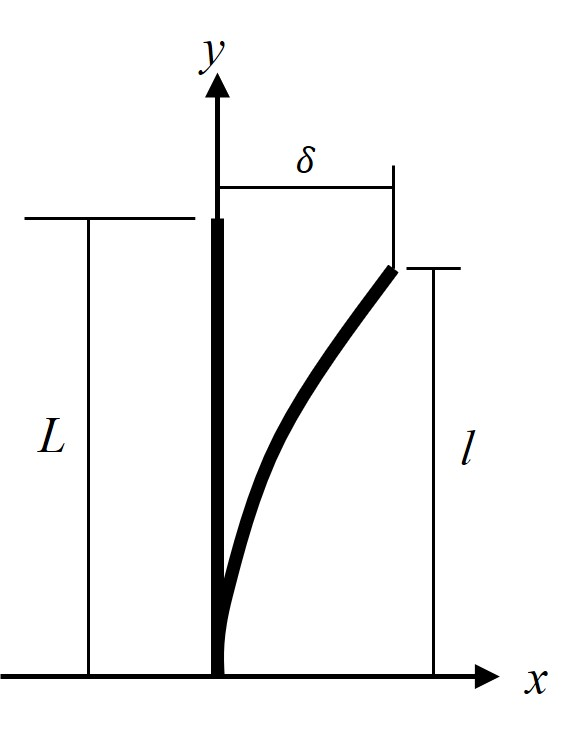
\includegraphics{FIG/bendingModel.jpg}}
  \caption{Bending of flexible canopy element.}
\label{fig:bend}
\end{figure}







\bibliographystyle{jfm}
% Note the spaces between the initials
\bibliography{jfm-instructions}

\end{document}
